%----------------------- Wydruk dwustronny ---------------
%\documentclass[12pt,twoside,a4paper]{book} % 
%----------------------- Wydruk jednostronny ---------------
\documentclass[12pt,oneside,a4paper]{book} % jednostronnego

\usepackage{polski}
\usepackage[utf8]{inputenc} %opcja dla edytorów kodujących polskie znaki w utf8
%\usepackage[cp1250]{inputenc} %opcja dla edytorów kodujących polskie znaki w windows-1250
\usepackage{lmodern}
\usepackage{indentfirst}
\usepackage[protrusion=false]{microtype}
\DisableLigatures{encoding = *, family = * }
\usepackage{fancyhdr}
\usepackage{pstricks,graphicx}
\usepackage{amssymb}
\usepackage{float}

\usepackage{pdflscape}
\usepackage{diagbox}

%---------------Zbiory liczbowe
\newcommand{\R}{\mathbb{R}}
\newcommand{\N}{\mathbb{N}}
\newcommand{\K}{\mathbb{K}}
\newcommand{\C}{\mathcal{C}}
\newcommand{\p}{\mathcal{P}}
%------------kwantyfikatory--------------
\newcommand{\fal}{\mbox{{\Large $\forall\,$}}}
\newcommand{\ext}{\mbox{{\Large $\exists\,$}}}
%------------------definicje środowisk-----------------
\usepackage{theorem}
\theoremstyle{break}
\theorembodyfont{\it}
\newtheorem{twr}{Twierdzenie}[chapter]
\newtheorem{lem}{Lemat}[chapter]
\theorembodyfont{\rm}
\newtheorem{defi}{Definicja}[chapter]
\newtheorem{wni}{Wniosek}[chapter]
\newtheorem{prz}{Przykład}[chapter]
\newenvironment{dowod}{\par\vspace{0.1cm}\par{ \sc Dowód.}}{\hfill $\blacksquare$\par\vspace{0.4cm}\par}
% ----------ustawienia wymiarow strony
\usepackage{geometry}

\newgeometry{tmargin=2.5cm, bmargin=2.5cm, headheight=14.5pt, inner=3cm, outer=2.5cm} 

\linespread{1.1} %-zmiana interlinii


\fancypagestyle{mylandscape}{
\fancyhf{} %Clears the header/footer
\fancyfoot{% Footer
\makebox[\textwidth][r]{% Right
  \rlap{\hspace{.75cm}% Push out of margin by \footskip
    \smash{% Remove vertical height
      \raisebox{4.87in}{% Raise vertically
        \rotatebox{90}{\thepage}}}}}}% Rotate counter-clockwise
\renewcommand{\headrulewidth}{0pt}% No header rule
\renewcommand{\footrulewidth}{0pt}% No footer rule
}

%---------------- Normalne środowiska --------------------
\usepackage{amsmath}

%----------nagłowki i żywa pagina ------------
\pagestyle{fancy} 
%--------------- Wydruk dwustronny
%\cfoot[]{} 
%\lhead[{\scriptsize{\it \thepage}}]{}
%\chead[{\scriptsize\leftmark}]{{\scriptsize \rightmark}}
%\rhead[]{{\scriptsize{\it \thepage}}}
%--------------- Wydruk jednostronny
\fancyhead[C]{} 
\fancyfoot[C]{\thepage}
\fancyhead[L]{\scriptsize\leftmark}
\fancyhead[R]{\scriptsize\rightmark}

\renewcommand{\chaptermark}[1]{%
\markboth{\MakeUppercase{%
\chaptername}\ \thechapter.%
\ #1}{}}

\usepackage[most]{tcolorbox}
\let\includegraphicsold\includegraphics
\newcommand{\includegraphicsborder}[2][]{\tcbox{\includegraphicsold[#1]{#2}}}

\renewcommand{\sectionmark}[1]{\markright{\thesection.\ #1}}

\usepackage[hidelinks]{hyperref}

\usepackage{graphics}
\graphicspath{ {images/} }

\usepackage{listings}

\renewcommand{\lstlistlistingname}{Spis listingów}
\renewcommand{\lstlistingname}{Listing}

\lstset{
  basicstyle=\footnotesize
}

\usepackage{booktabs}

\newcommand\tabularhead[2]{
  \begin{table}[ht]
    \label{#2}
    \caption{#1}
    \begin{tabular}{|p{0.35\linewidth}|p{0.6\linewidth}|}
    \hline
    \textbf{#1}\\
    \hline
}
\newcommand\addrow[2]{#1 &#2\\ \hline}

\newcommand\addmulrow[2]{ \begin{minipage}[t][][t]{2.5cm}#1\end{minipage}
   &\begin{minipage}[t][][t]{8cm}
    \begin{enumerate} #2   \end{enumerate}
    \end{minipage}\\ }

\newenvironment{usecase}{\tabularhead}
{\hline\end{tabular}\end{table}}



%-----------------właściwa część pracy-----------------
\begin{document}
\thispagestyle{empty}
\begin{center}
  \Large
  \bf{UNIWERSYTET ŚLĄSKI}\\
  \bf{\sf{WYDZIAŁ NAUK ŚCISŁYCH I TECHNICZNYCH}}\\[25mm]
  \large

  \bf{Przygotowanie danych w Rapid Miner}\\[35mm]

  Sprawozdanie\\
  z przedmiotu\\
  Eksploracja Danych\\[25mm]
\end{center}
\begin{flushright}
  \large
  Autorzy:\\
  Kacper Małachowski\\
  grupa 3, I rok\\[25mm]
\end{flushright}

\chapter*{Źródło danych}

Dane pochodzą z repozytorium uniwersytetu kalifornijskiego, gdzie znajdują się pod nazwą "Room Occupancy Estimation".
Stworzone zostały w ramach badań: Adarsh Pal Singh, Vivek Jain, Sachin Chaudhari, Frank Alexander Kraemer, Stefan Werner and Vishal Garg, "Machine Learning-Based Occupancy Estimation Using Multivariate Sensor Nodes," in 2018 IEEE Globecom Workshops (GC Wkshps), 2018.

\subsection*{Opis atrybutów}

\begin{itemize}
  \item Date - Pominięty w eksploracji - Data pomiaru z czujników.
  \item Time - Pominięty w eksploracji - Czas pomiaru z czujników z dokładnością do sekund.
  \item S1\_Temp - Odczyt z czujnika temperatury umieszczonego przy biurku nr 1, podany w stopniach celsjusza.
  \item S2\_Temp - Odczyt z czujnika temperatury umieszczonego przy biurku nr 2, podany w stopniach celsjusza.
  \item S3\_Temp - Odczyt z czujnika temperatury umieszczonego przy biurku nr 3, podany w stopniach celsjusza.
  \item S4\_Temp - Odczyt z czujnika temperatury umieszczonego przy biurku nr 4, podany w stopniach celsjusza.
  \item S1\_Light - Odczyt z czujnika światła umieszczonego przy biurku nr 1, podany w luxach.
  \item S2\_Light - Odczyt z czujnika światła umieszczonego przy biurku nr 2, podany w luxach.
  \item S3\_Light - Odczyt z czujnika światła umieszczonego przy biurku nr 3, podany w luxach.
  \item S4\_Light - Odczyt z czujnika światła umieszczonego przy biurku nr 4, podany w luxach.
  \item S1\_Sound - Odczyt z przetwornika analogowo-cyfrowego podłączonego do wyjścia wzmacniacza mikrofonu, wyrażony w woltach. Czujnik ten umieszczony jest przy biurku nr 1.
  \item S2\_Sound - Odczyt z przetwornika analogowo-cyfrowego podłączonego do wyjścia wzmacniacza mikrofonu, wyrażony w woltach. Czujnik ten umieszczony jest przy biurku nr 2.
  \item S3\_Sound - Odczyt z przetwornika analogowo-cyfrowego podłączonego do wyjścia wzmacniacza mikrofonu, wyrażony w woltach. Czujnik ten umieszczony jest przy biurku nr 3.
  \item S4\_Sound - Odczyt z przetwornika analogowo-cyfrowego podłączonego do wyjścia wzmacniacza mikrofonu, wyrażony w woltach. Czujnik ten umieszczony jest przy biurku nr 4.
  \item S5\_CO2 - Odczyt z detektora CO2, umieszczonego na środku pokoju, wyrażony w cząsteczkach na milion.
  \item S5\_CO2\_Slope - Zmiana stężenia CO2 w pomieszczeniu z detektora umieszczonego na środku pomieszczenia.
  \item S6\_PIR - Wartość prawda-fałsz wskazująca na wykrycie ruchu przez czujnik umieszczony nad drzwiami.
  \item S7\_PIR - Wartość prawda-fałsz wskazująca na wykrycie ruchu przez czujnik umieszczony na ścianie na przeciwko drzwi.
\end{itemize}

\chapter*{Projekt w Rapid Miner}

Ponizej przedstawiono zdjęcie projektu z programu Rapid Miner.

\begin{figure}[H]
  \centering
  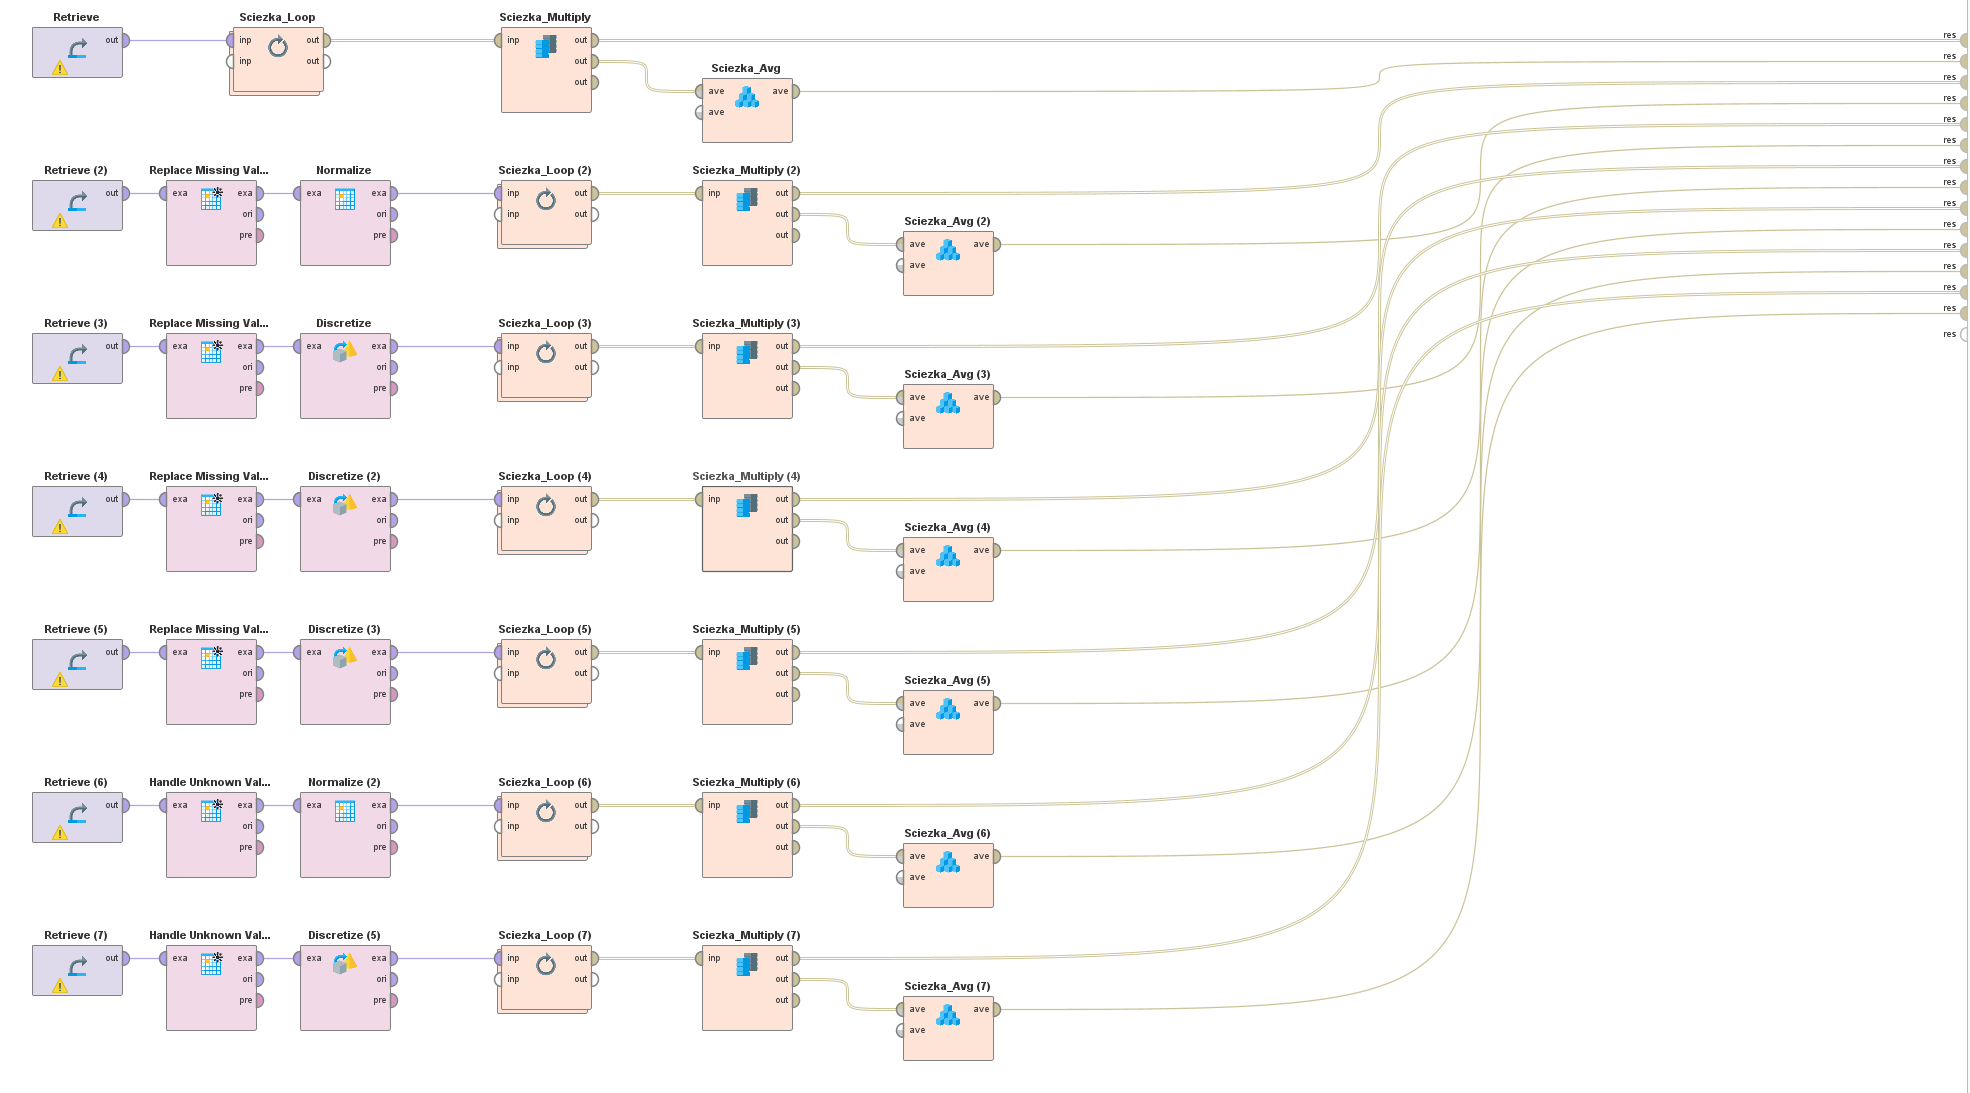
\includegraphics[width=1\textwidth]{whole-project.png}
\end{figure}
\begin{figure}[H]
  \centering
  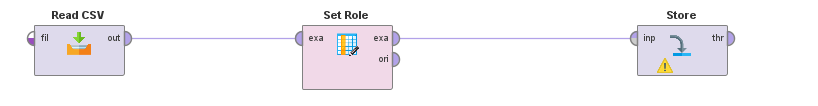
\includegraphics[width=0.75\textwidth]{loading-project.png}
\end{figure}

\subsection*{Opis składowych projektu}

Projekt podzielono na dwa procesy, jeden wczytujący dane z pliku .csv do lokalnego repozytorium oraz drugi określający skuteczność dla poszczególnego przygotowania danych.

\subsubsection*{Wczytanie danych do repozytorium}

Dane zostały wstępnie przygotowane poprzez usunięcie ok. 9.5\% danych z dwóch kolumn.
Były to kolumny S4\_Sound oraz S5\_CO2\_Slope, wykonano to z uwagi na fakt, że dane źródłowe nie posiadały brakujących wartości. Dane zostały usunięte przy pomocy specjalnie przygotowanego skryptu w języku python, dla zapewnienia losowości.

Proces wczytania danych składa się z trzech operatorów:

\begin{itemize}
  \item Read CSV - w którym ustawiono ścieżkę do pliku z brakujacymi danymi znajdującego się na lokalnym dysku. Jako separator kolumn pozostawiono domyślny przecinek, pozostałych opcji również nie modyfikowano. W procesie wczytywania danych wykluczono kolumny odpowiedzialne za datę i czas oraz zmieniono typ kolumny "Room Occupancy Count" na polynominal z domyślnej liczby całkowitej.
  \item Set Role - operator służy to ustawienia roli kolumny "Room Occupancy Count" na wartość label.
  \item Store - W operatorze ustawiono ścieżkę zapisu danych w lokalnym repozytorium dla rapid minera.
\end{itemize}

\subsubsection*{Proces przygotowania i analizy danych}

Omówienie parametrów dla tego procesu zostanie podzielone na dwie części, pierwszą wspólną dla wszystkich ścieżek obejmujacą wczytanie danych z repozytorium i ich walidacje oraz drugą charakterystyczną dla poszczególnych ścieżek polegającą na przygotowaniu danych.

Pierwszym wspólnym elementem dla wszystkich ścieżek jest wczytanie danych, którego jedyną ustawioną opcją jest ścieżka do danych w lokalnym repozytorium programu Rapid Miner.

Kolejnymi elementami wspólnymi dla wszystkich ścieżek jest złożony operator pętli. W operatorze tym ustawiono liczbę iteracji na 20. Natomiast wewnatrz tego operatora znajduje się operator walidacji krzyżowej z wartością wykonań ustawioną na 10. Podział próbek wykonywany jest automatycznie.

W sekcji treningowej umieszczono model drzewa decyzyjnego z kryterium ustawionym na "gain\_ratio" z maksymalną głębokoscią ustawioną na 10. "Confidence" ustawiono na 0.1, "minimal gain" na 0.01, a minimalnawielkosć liścia na 2.

W sekcji testowej, umieszczono operator apply model otrzymujący wytrenowany model oraz dane testowe. Pondato umieszczono tutaj również operator "Prefromance" obliczajacy skuteczność modelu.

Za pętlą umieszczono jeszcze dwa operatory, pierwszy "multiply" powiela wyniki z pętli, jedne trafiają bezposrednio na wyjście. Drugie zaś trafiają do operatora "Average", który oblicza średnią dokładność z otrzymanych 20 iteracji pętli.

Pierwsza ścieżka stanowi punkt odniesienia dla pozostałych i nie zawiera operatorów przygotowywujących dane.

Druga ścieżka do przygotowania danych używa operatora "Replace Missing Values", który działa na wszystkich atrybutach ("attrubute filter type" ustawiony na "all") oraz używa średniej wartości do zastąpienia brakujacych wartości. Drugim krokiem jest normalizacja wszystkich atrybutów ("atrubute filter type" ustawiony na "all").

Trzecia ścieżka używa również operatora "Replace Missing Values" na wszystkich atrybutach, ale zamiast sredniej zastępuje je zerami. Ponadto używa dyskretyzacji z parametrami "attribute filter type" ustawionym na "all" oraz "number of bins" ustawionym na 2.

Czwarta ścieżka również używa operatora "replace Missing Values" dla wszystkich atrybutów, ale używa wartości maksymalnej do zastąpienia brakujacych wartości.
Pondato przeprowadzona ona dyskretyzacje na kolumnie "S1\_Light" ("attribute filter type" z wartoscią "single" oraz "attribute" z wartością "S1\_Light") z domyślną wartością atrybutu "number of bins".

Piąta ścieżka podobnie jak poprzednie używa operatora "Replace Missing Values" to zastąpienia brakujących wartości, ale zastępuje je wartościami minimalnymi. Podobnie jak w ścieżce czwartej następuje dyskretyzacja na pojedynczej kolumnie, z tą różnicą że jest to kolumna "S5\_CO2".

Szósta ścieżka używa operatora "Handle Unknown Values" z parametrem "attribute filter type" ustawionym na "all". Ponadto używa ona normalizacji również z parametrem "attribute filter type" ustawionym na "all".

Siódma ścieżka używa operatora "Handle Unknown Values" z takimi samymi parametrami jak ścieżka szósta, ale używa dyskretyzacji z parametrami "attribute filter type" z wartoscią "all" oraz "number of bins" z wartością 2.

\begin{landscape}
\thispagestyle{mylandscape}
\chapter*{Wyniki walidacji krzyżowej}

W poniższej tabeli przedstawiono wyniki walidacji krzyżowej dla poszczególnych ścieżek i iteracji pętli. Wyniki wyrażone są jako procent dokładności modelu.

\begin{table}[H]
  \resizebox{1.5\textwidth}{!}{
  \begin{tabular}{|c|c|c|c|c|c|c|c|c|c|c|c|c|c|c|c|c|c|c|c|c|c|c|}
  \hline
  \backslashbox{Ścieżka}{Iteracja}  & 1 & 2 & 3 & 4 & 5 & 6 & 7 & 8 & 9 & 10 & 11 & 12 & 13 & 14 & 15 & 16 & 17 & 18 & 19 & 20 & Średnia \\ \hline
   1  & 98.70\% & 98.61\% & 98.52\% & 98.74\% & 98.60\% & 98.66\% & 98.51\% & 98.52\% & 98.69\% & 98.65\% & 98.73\% & 98.63\% & 98.56\% & 98.55\% & 98.53\% & 98.67\% & 98.46\% & 98.57\% & 98.70\% & 98.53\% & 98.63\% \\ \hline
   2  & 98.70\% & 98.82\% & 98.70\% & 98.70\% & 98.80\% & 98.69\% & 98.70\% & 98.77\% & 98.59\% & 98.68\% & 98.81\% & 98.74\% & 98.77\% & 98.70\% & 98.80\% & 98.77\% & 98.93\% & 98.75\% & 98.88\% & 98.92\% & 98.72\% \\ \hline
   3  & 91.94\% & 91.91\% & 91.86\% & 91.93\% & 91.85\% & 91.95\% & 91.88\% & 91.98\% & 91.98\% & 91.87\% & 91.93\% & 91.89\% & 91.93\% & 91.89\% & 91.90\% & 91.98\% & 91.81\% & 91.85\% & 91.94\% & 91.92\% & 91.92\% \\ \hline
   4  & 98.25\% & 98.01\% & 97.95\% & 98.18\% & 98.05\% & 98.38\% & 98.40\% & 98.23\% & 98.26\% & 98.35\% & 98.07\% & 98.15\% & 97.97\% & 98.11\% & 98.26\% & 98.14\% & 98.21\% & 98.00\% & 98.15\% & 97.75\% & 98.18\% \\ \hline
   5  & 98.77\% & 98.78\% & 98.84\% & 98.84\% & 98.82\% & 98.81\% & 98.73\% & 98.84\% & 98.91\% & 98.91\% & 98.92\% & 98.75\% & 98.83\% & 98.92\% & 98.64\% & 98.84\% & 98.70\% & 98.71\% & 98.69\% & 98.90\% & 98.79\% \\ \hline
   6  & 98.57\% & 98.52\% & 98.68\% & 98.65\% & 98.45\% & 98.56\% & 98.59\% & 98.52\% & 98.59\% & 98.76\% & 98.58\% & 98.55\% & 98.69\% & 98.72\% & 98.72\% & 98.54\% & 98.68\% & 98.57\% & 98.74\% & 98.53\% & 98.60\% \\ \hline
   7  & 91.92\% & 91.93\% & 91.95\% & 91.97\% & 91.79\% & 91.86\% & 91.93\% & 91.81\% & 91.88\% & 92.00\% & 91.87\% & 91.89\% & 91.89\% & 92.05\% & 91.93\% & 91.95\% & 91.90\% & 91.99\% & 91.92\% & 91.88\% & 91.92\% \\ \hline
  \end{tabular}}
  \end{table}

\end{landscape}

\chapter*{Wnioski}

Jak można zobaczyć po wynikach walidacji modelu, najlepszy wynik uzyskano na ścieżkach nr 2 oraz 5. Na podsatwie powyższych wyników, stwierdzić można że przygotowanie danych wykazuje poprawę względem danych nieprzygotowanych, a dyskretyzacja przy odpowiednio dobranej kolumnie danych pozwala uzyskać lepsze wyniki niż możnaby uzyskać przy pomocy normalizacji.

Zwrócić należy uwagę na fakt, że dyskretyzacja znacząco pogorszyła ocenę jakości w przypadku gdy brakujace wartości zastąpiono zerami. W pozostałych przypadkach natomiast wartości te nie odbiegają znacząco od siebie.

Pondato na podstawie powyższych danych wysnuć należy wniosek, że odpowiedni dobór atrybutów poddanych dyskretyzacji pozwala uzyskać lepsze wyniki niż przeprowadzenie dyskretyzacji na całym zbiorze atrybutów.

Ostatecznie przygotowanie danych przed ich wykorzystaniem pozwala uzyskać znacząco lepsze rezultaty niż korzystanie z danych surowych. W świecie cyfryzacji, przygotowanie nawet dużych zbiorów danych nie stanowi zazwyczaj wyzwania. Przynajmniej nie stanowi wyzwania, które usprawiedliwia wykorzystanie surowego zbioru danych podczas analizy.

\end{document}